there are three different models considered. The first one is magnetic elastic actuator; it utilizes magnetic field generated by the solenoid to move a ferromagnetic bar equipped with a surrounding spring. When there is a current acted, the bar is attracted inside the hall of the solenoid and the spring, wrapped around the bar, is compressed.
When there is no current the bar is released, and the spring maintains pin's position. This model is safe, simple to replicate and the cheapest solution with an estimated cost of USD 40 per cell.
Besides, it also has the potential to be converted into large area dense array display, which satisfies our goal. The other two models are magnetic linear actuators and magnetic rail, which are more or less similar to the working principle of the first one, but they are also eliminated because the either high error rate or relatively high cost compared to the elastic actuator.

\begin{figure} \centering
    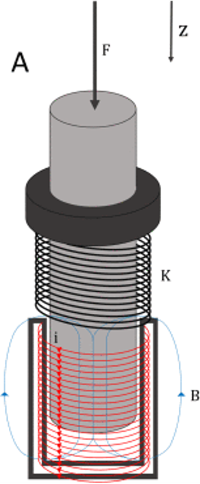
\includegraphics[height=5cm]{figures/magnetic-spring.png}
\caption{A single solenoid with the ferromagnetic element and the linear spring (elastic constant k). A current i flows in the red solenoid and generates a magnetic field B. The bar is then attracted downwards with a force F .}
\label{fig:magnetic-spring.png}
\end{figure}

\paragraph{Ferromagnetic fluids}
Despite its early developmental stage, the use of ferromagnetic fluids is promising \cite{fletcher_magnetic_2021}.
Character in a cell are individually created by their correspondent electromagnet, and can reasonably meet the UK Association for Accessible Formats (UKAAF) standards.
Given it is at a proof-of-concept stage, producing it for this study is unreasonable.